 
\documentclass[11pt,twocolumn]{article}

    \usepackage{fullpage}          %This will give you the standard 1in. margins, 12pt font, single spaced, page numbers, ect.  
    \usepackage{url}                 %This is intended if you have a website in the bibliography
    \usepackage{graphicx}         %This is if you want to include a picture in your document


    \usepackage{amsmath, amsthm, amssymb}
    \usepackage{epsfig}
    \usepackage{pslatex}
     

    \title{Techniques for Fractal Terrain Generation}
    \author{Krista Bird \and Thomas Dickerson \and Jessica George}
    \begin{document}
    \maketitle

    \begin{abstract}
    In this paper we present various methods of fractal terrain generation.
	We discuss the relative advantages and disadvantages of each method. Methods presented include: midpoint displacement,
	Fourier space manipulation of gaussian noise, multi fractal methods, and their respective variations. 
    \end{abstract}
     
    \section{Introduction}
	\label{sec:intro}
	The work discussed in this paper aims to describe different methods and algorithms that are used for artificial fractal
	landscape generation.  The goal in generating these landscapes is to make them look as realistic as possible.
	To make a terrain look realistic there are many different aspects that need to be taken into consideration.
	Some of these include hills and valleys, color, trees and other plants. The focus of this paper is going to be
	on different methods used to generate the terrain and how realistic they look based on the hills and valleys. The
	algorithms discussed in this paper all have varying levels of accuracy when it comes to representing the topological
	aspect of the landscape naturally. 

	Fractal geometry is a branch of mathematics that studies irregular shapes in the real world. The general definition of a
	fractal is an infinitely self-similar, iterated, and detailed mathematical shape with a non-integer dimension. More simply,
	fractals are shapes that have self-similar patterns, meaning that they appear to look the same far away as they do up close.
	Fractals can first be seen in mathematics as early as the 17th century with the idea of recursion.  The word `fractal' was not
	introduced until 1975 by a mathematician named Benoit Mandelbrot. It is derived from the Latin word fractus, which means broken
	or shattered glass. 

	\begin{figure}[ht]
	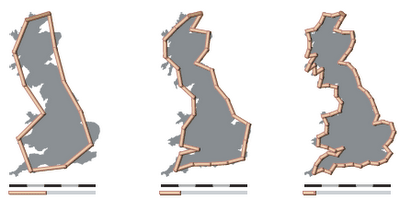
\includegraphics[scale=0.5]{BritainCoastline.png}
	\caption{The coastline of Britain has a fractal dimension}
	\label{fig:britcoast}
	\end{figure}
	Fractals were first used in terrain generation in 1967. Benoit Mandlebrot was the mathematician to first propose it.
	Mandlebrot proposed a question concerning the length of the British coastline.  This simple question
	lead to many different and varying results. This is because it depended on the scale that the person was using to measure the
	coastline (see Figure \ref{fig:britcoast}). Examining the coastline at increasingly higher resolutions yields an increase in
	length due to the recursive levels of detail. The answer to the question is that the coastline of Britain is not measurable because
	it is not one-dimensional. It is a fractal. ~\cite{Mandelbrot}.

	Fractals are used in landscape generation because they are self-similar and have a non-integer dimension. Being self-similar means
	that the fractal is going to appear basically the same no matter the level of magnification. So fractals are able to produce a landscape
	that is going to look like a terrain no matter the level of magnification. Fractals are also optimal for landscape generation because of
	their non-integer dimensions. This means that fractals have a dimension that is between two whole numbers. A fractal will vary between
	these two whole numbers depending on how much space it needs as it twists and curves. This means that a fractal that is closing in on
	two dimensions is going to appear as a large hill with small mounds and a fractal approaching three dimensions is going to resemble a
	rougher terrain with slightly smaller hills. ~\cite{Mandelbrot}.

	\S \ref{sec:midpoint} explores is the Midpoint Displacement Algorithm. The algorithm is the simplest algorithm for generating terrain.
	The Midpoint Displacement algorithm was introduced in [some year].

	Another method that is similar to, but not exactly the same as, the Midpoint Displacement Algorithm is the Diamond Square Algorithm.
	Alain Fournier, Don Fussell, and Loren Carpenter first described the Diamonds \& Squares Algorithm at SIGGRAPH 1982 (Special Interest
	Group on GRAPHics and Interactive Techniques). Gavin S. P. Miller revisited this algorithm in 1986 at the same conference. This is when
	it was discovered that the algorithm was �flawed�. The algorithm produces vertical and horizontal creases in the generated landscape.
	~\cite{Miller}.

	Both the Diamond-Square Algorithm and the Midpoint Displacement Algorithm use multiple iterations of random values to create a landscape.
	This is going to apply the iteration at a smaller scale each time through. It will then take the random number as an altitude to produce
	the resulted landscape. Both of these algorithms use recursive subdivision methods, which allows both of these algorithms to be run in
	linear time. ~\cite{Miller}.

	\S \ref{sec:FFT} describes the use of the Fast Fourier transformation can be used to create fractal landscapes as well.
	This is going to create a landscape using a frequency domain. The landscape generated by this algorithm is going to take
	in the random numbers and model their frequencies to create a landscape. ~\cite{Kareem}.
	
	Finally, \S \ref{sec:multifractal} describes the multifractal and its application to terrain generation. A multifractal
	set is a set of fractals that can be divided up into multiple subsets, each having their own dimension. A multifractal
	system is different from a fractal system because it has more than just one exponent. A multifractal system is used when
	more than one exponent is needed to describe the dynamics of an object. This can be seen in terrain generation. They allow
	for a more precise and natural looking landscape as the magnification is increased. 

	In the remainder of this paper we will explore the three methods mentioned above: the Midpoint Displacement Algorithm (and the
	Diamond Square Algorithm), the Fast Fourier Transformation Algorithm, and the Multifractal technique, in more detail. We will
	also discuss the implementation of each of these methods and examine the resulting landscapes. 
	

	\section{Midpoint Displacement Method}
	\label{sec:midpoint}
		Generating fractal terrains by midpoint displacement is a relatively straightforward method for generating artificial terrain with realistic features. The dimensions of the terrain must be a square with sides of length $2^{N}+1$, so that each sub-square has an exact middle lying on a gridpoint. Given a heightfield,
		\begin{equation}
		T = \left[ \begin{matrix}
		T_{0,0} & \ldots & T_{0,2^{N},} \\
		\vdots  &  \ddots & \vdots \\
		T_{2^{N},0} & \ldots & T_{2^{N},2^{N}}
		\end{matrix} \right]
		\end{equation}
then for midpoints along columns,
		\begin{equation}
			T_{k \cdot 2^{n},j \cdot 2^{n}} = \frac{T_{(k+1) \cdot 2^{n},j \cdot 2^{n}} + T_{(k-1) \cdot 2^{n},j \cdot 2^{n}}}{2} + A \cdot R \cdot 2^{-H \cdot n}
		\end{equation}
and similarly, for midpoints along rows,
		\begin{equation}
			T_{j \cdot 2^{n},k \cdot 2^{n}} = \frac{T_{j \cdot 2^{n},(k+1) \cdot 2^{n}} + T_{j \cdot 2^{n},(k-1) \cdot 2^{n}}}{2} + A \cdot R \cdot 2^{-H \cdot n}
		.\end{equation}
Whereas midpoints centered between corners are given by
				\begin{equation}
			%T_{k \cdot 2^{n},k' \cdot 2^{n}} = \frac{T_{(k-1) \cdot 2^{n},(k'-1) \cdot 2^{n}} + T_{(k-1) \cdot 2^{n},(k'+1) \cdot 2^{n}} + T_{(k+1) \cdot 2^{n},(k'-1) \cdot 2^{n}} + T_{(k+1) \cdot 2^{n},(k'+1) \cdot 2^{n}}}{4} + A \cdot R \cdot 2^{-H \cdot n}
			\begin{split}
			T_{k \cdot 2^{n},k' \cdot 2^{n}} =& \left(\frac{1}{4}\right)T_{(k-1) \cdot 2^{n},(k'-1) \cdot 2^{n}} \\
			& + \left(\frac{1}{4}\right)T_{(k-1) \cdot 2^{n},(k'+1) \cdot 2^{n}} \\
			& + \left(\frac{1}{4}\right)T_{(k+1) \cdot 2^{n},(k'-1) \cdot 2^{n}} \\
			& + \left(\frac{1}{4}\right)T_{(k+1) \cdot 2^{n},(k'+1) \cdot 2^{n}} \\
			& + A \cdot R \cdot 2^{-H \cdot n}
			 \end{split}
		.\end{equation}
(where
		\begin{equation}
			k,k' \in \left\{ 1, 3, \cdots, 2^{N-n}-1 \right\}
		\end{equation}
and
		\begin{equation}
			m \in \left\{ 0, 2, \cdots, 2^{N-n} \right\}
		\end{equation})
for $n < N$ and $m \in \mathbb{Z}$. H is a smoothing parameter, A is an amplitude parameter, and R is a random number from a uniform distribution between -1 and 1.
 \begin{figure}[ht]
  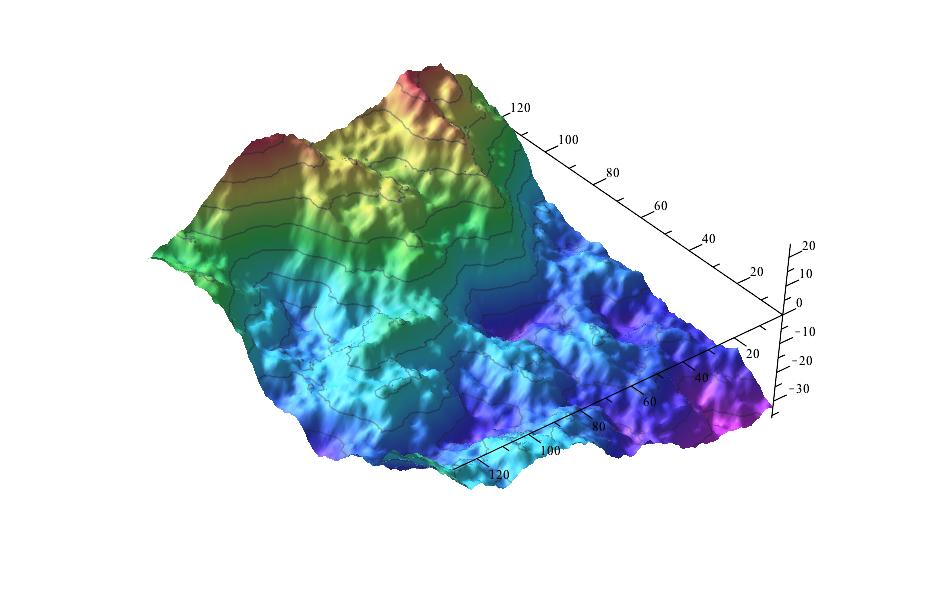
\includegraphics[scale=0.25]{midpoints.jpg}
  \caption{An artificial terrain generated using the Midpoint Displacement Algorithm}
  \label{fig:midpoint}
  \end{figure}


	\subsection{Variations: Diamands and Squares}
	One criticism of the realism of the terrain generated by Midpoint Displacement is that it sometimes
	leaves square-shaped artifacts in the terrain. The Diamonds and Squares method attempts to alleviate this
	by alternating calculated values to square and diamond patterned midpoints. 
		
	\begin{figure}[ht]
	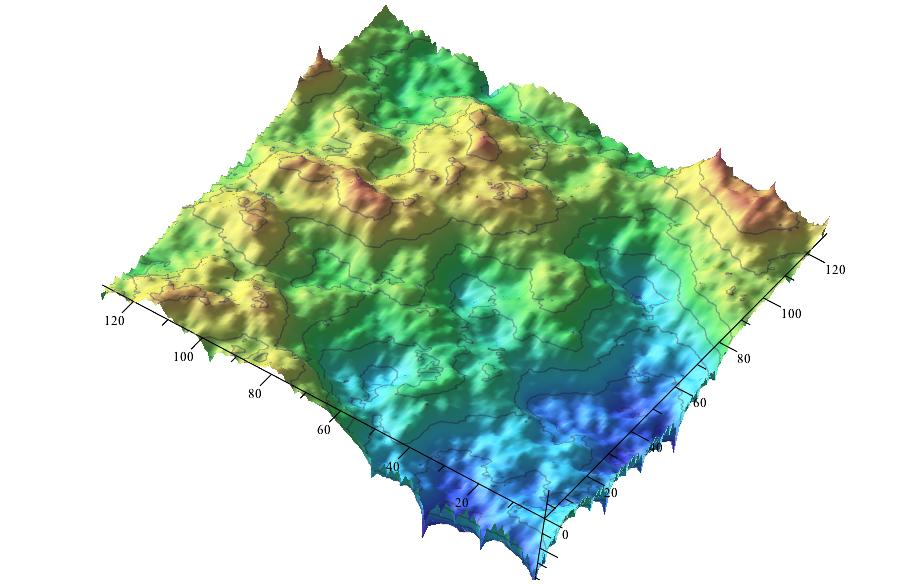
\includegraphics[scale=0.25]{diamondsandsquares.jpg}
	\caption{An aritifical terrain generated using the Diamond and Squares Algorithm}
	\label{fig:DandS}
	\end{figure}
  
	\subsection{Implementation Challenges}
	Maple has a very small limit on stack space for use by recursively defined functions, so the algorithm must be rewritten as an iterative one.
	Additionally, Maple uses 1-indexed arrays, which makes a few formulas slightly bulkier.

	\section{Using the Fast Fourier Transform to Generate Fractal Terrain} 
	\label{sec:FFT}
	In 1965, J.W. Cooley and J.W. Tukey published the fast Fourier transform algorithm.
	This algorithm made it possible to calculate the discrete Fourier transform using multiple operations
	in time $O(NlogN).$ The fast Fourier transform makes it possible for us to generate a fractal terrain.
	A Fourier transform is another method to generate fractal terrains. This is generally used to generate
	older terrains with a flatter landscape. The landscape created by a Fourier transform can be tiled.
	The Fourier transform enables us to express random noise as a function of sine and cosine functions,
	and it converts the function to a frequency domain. The result is a fractal landscape with smooth rolling
	features rather than ridges and peaks that can be generated using other methods. Thus, the landscape is a sum
	of the sine and cosine waves at different frequencies.
	
	Unlike many other processes for fractal terrain generation, the Fourier method is not an iterative process ~\cite{Kareem}.
	Initially, we begin using a random Gaussian noise (other types of noise can be used here as well), which is a two dimensional
	grid of discrete random values. Using Maple, we are able to apply the fast Fourier transform (FFT), which preforms a discrete
	Fourier transform (DFT). A two dimensional discrete Fourier transform for and $N$x$M$ grid in the $x$, $y$ plane is 
	$$F(u,v)=\frac{1}{NM}\displaystyle\sum\limits_{x=0}^{N-1} \displaystyle\sum\limits_{y=0}^{M-1} f(x,y)e^{-2\pi i(xu/N+yu/M)},$$
	and the inverse is
	$$f(x,y)=\displaystyle\sum\limits_{u=0}^{N-1} \displaystyle\sum\limits_{v=0}^{M-1} F(u,v)e^{2\pi i(xu/N+yv/M)}.$$ ~\cite{CooleyTukey}.

	The FFT allows us to decompose the random noise into the sum of the sine and cosine functions. In Fourier space, the noise is broken
	into cells. Within each cell, we can find the magnitude of the wave with that frequency. These magnitudes are then be converted to
	the frequency domain. In this domain, each frequency is a complex number. This is all done through the use of the FFT algorithm.
	
	Once the values are in the frequency domain, we must scale these frequencies because we will have some that are very high and
	some that are very low. We do this using a frequency filter of the form $1/f^{r}$. The $f$ is the frequency represented by that
	value and the $r$ is a roughness parameter. After we have scaled the frequencies we can apply an inverse fast Fourier transform
	in order to generate a fractal landscape that is the sum of the waves at different frequencies. This is the source of the landscape's
	"rolling" quality ~\cite{Kareem}. We apply this FFT to a two diminutional random noise, but we are able to view the data in three
	dimensions. The result is a fractal landscape. There are no artificial ridges or peaks and the landscape is easily tiled.
	
	The characteristics of the landscape are determined by the random seed number. How rough or smooth the surface of the landscape
	is depends on the value you scale the frequencies by. The higher the number you scale by the smoother the landscape. The smaller
	the scaling number, the rougher the landscape. Though we can change the relative roughness of the terrain the landscape will have
	a smooth surface in comparison to the previous methods we described.  

	\begin{figure}[ht]
	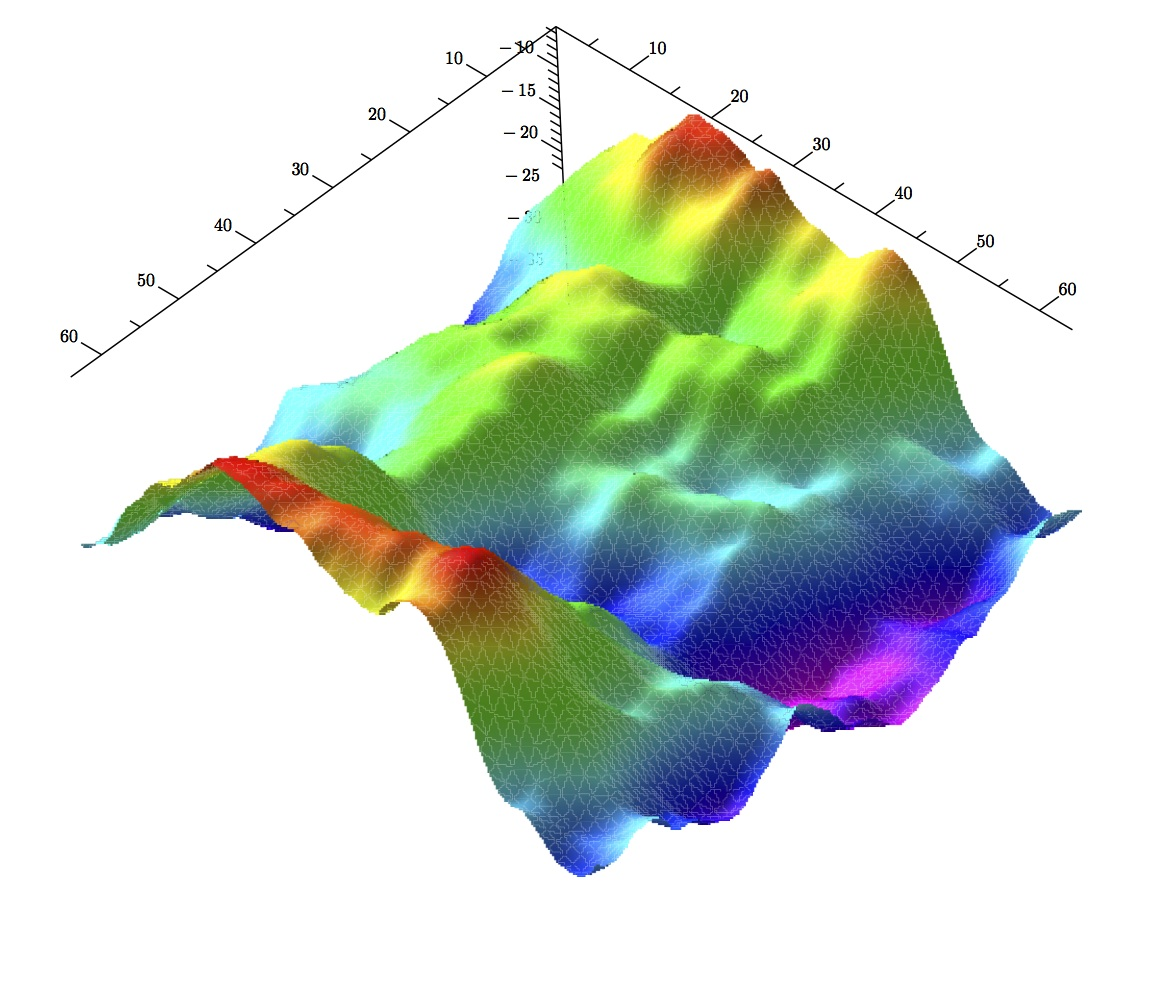
\includegraphics[scale=0.35]{FourierLandscape.jpg}
	\caption{An artificial terrain generated using the Fast Fourier Transform}
	\label{fig:fourier}
	\end{figure}

	\section{Multifractal Technique}
	\label{sec:multifractal}
	Multifractal technique is an extremely recent technique in generating terrain. This technique so far has mostly been used to
	extract information for images of natural terrain. It then takes this information extracted from the image and create a generated
	landscape matching the natural landscape in the picture. This technique has been used in SAR (Synthetic Aperture Radar) imaging
	for generating what the terrain on Mars and other planets look like. However, this technique can be applied to generating a whole
	new terrain that is not based of an image.  This is what makes the multi fractal technique valuable technique, it can be used to
	extract information from an actual terrain to make a generated duplicate of it and it can generate terrain from scratch without
	using an image.
		
	The multi fractal technique uses four parameters to create a generated landscape. These four variables are: $\alpha$, $C1$, $S$,
	and $R$. The variable $\alpha$ is the Levy parameter that is used to determine the occurrence of peaks or singularities in the
	terrain. The variable $C1$ is the parameter that controls the spareness of the mean terrain height, or more simply put the
	roughness of the terrain.The variable $S$ is used as a seed (an initial number) for the random number generator. Lastly, $R$
	is for the square resolute of the terrain surface. ~\cite{PabstJense}.
	
	This technique uses a turbulent discrete cascade model. This model was originally used to model fluid flows.
	It applies the idea of singularities, which are sudden changes in the behavior of the turbulence, and applies it
	to the terrain. In a terrain, singularities can be modeled as mountain peaks. ~\cite{PabstJense}.
	
	There are four different stages that are used to create the final multi fractal generated terrain.
	The first stage in this process is creating the multi fractal field, $\epsilon$. To generate a multi-fractal
	field, is to use a Levy noise field. When generating a Levy noise field, there are two main parameters that control
	the outcome of the field produced. These two variables are $\alpha$ and $C1$. Both of these variables parameterized
	the equation $K(q)$, called the moment scaling function.  The fist variable, $\alpha$, is going to vary between 0 and 2.
	If $\alpha$ equals 2, there are going to be smaller peaks and valleys in the terrain. When $\alpha$ is less than 2,
	there are going to be bigger and more drastic peaks in the generated terrain. Once this $\alpha$ is selected,
	it is subsequently normalized. The second variable, $C1$, which controls the roughness of the terrain, is
	generated by the code-dimension of the mean of the field.
	
	The second stage in the multi fractal technique is to filter the terrain from stage one to get a multi-scaling
	behavior according to the characteristic function, $K(q)$.
	
	The four and final stage of creating this terrain, is taking that raw multi fractal field and fractal integrating it.
	This is going to take the raw field, which is has extreme pointed spikes throughout the field. The raw multi fractal
	field is unrealistic when it comes to terrain generation, unless it is modeling the inside of a cave. When the raw multi
	fractal field is integrated, it smoothes out the spikes and make the output look like an actual terrain. This resulting
	terrain after this stage is going to be the completed landscape generated by the multi fractal technique.

	\section{Our Artificial Three Dimensional Terrain}
	\label{sec:ourterrain}
	Another method to generate terrain is multiplying two methods together in rode to create a more realistic looking terrain.
	By using this method, it is possible to create flatter valleys and sharper peaks (see Figure \ref{fig:multiplication}). 

	\begin{figure}[ht]
	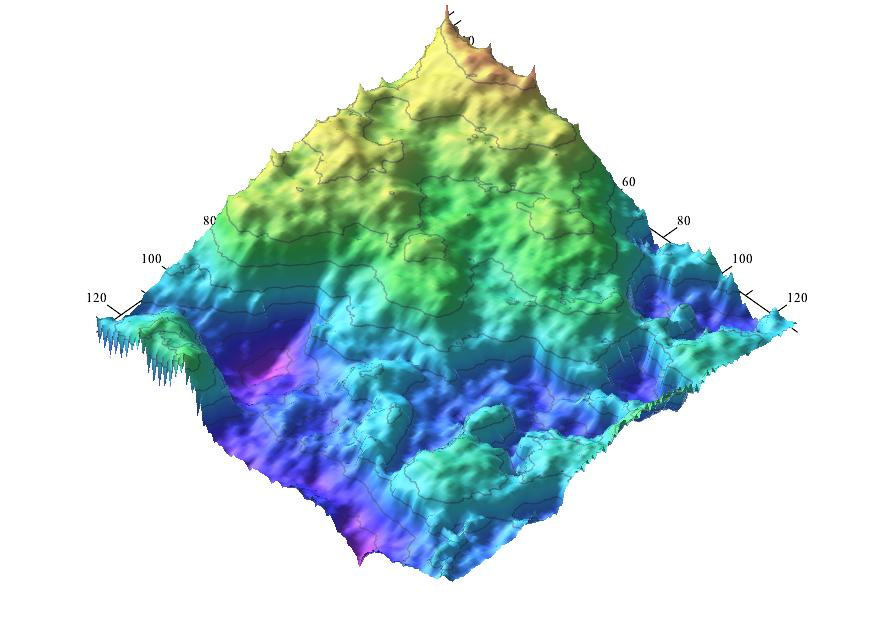
\includegraphics[scale=0.3]{multipliedterrain.jpg}
	\caption{A terrain generated using the Multiplication Method}
	\label{fig:multiplication}
	\end{figure}

	\section{Conclusion}
	\label{sec:conclusion}
	This paper has discussed and examined three different algorithms for generating fractal terrain.
	The Midpoint Displacement Algorithm and the Diamond Square Algorithm have been shown to be very similar.
	This is because the Diamond Square Algorithm is an improvement apron the Midpoint Displacement Algorithm.
	The two algorithms, in fact, only differ by one step that has been added to the Diamond Square Algorithm.
	They both produce terrain that is quantifiably different than natural terrains. It can be seen in the terrains
	generated that there are some obvious flaws. One of the biggest flaws of these two algorithms is that they produce
	`crease' in the terrain that is generated. These crease can either be vertical or horizontal, both of which help
	in making the terrain look unnatural. 
   
	The Fourier transformation, on the other hand, creates a landscape that is smoother than the terrain generated
	by the above two algorithms. The Fourier terrain produces terrain with flatter, rolling peaks and valleys. The peaks
	and the valleys produced by the Fourier transformation produce a smoother landscape with less exaggerated changes in
	the height. 
   
	The multifractal terrain generation is the most recent algorithm that was explored in this paper. This method of terrain
	generation aims to make the terrain look even more natural and not computer generated than the above two algorithms. This
	algorithm uses the idea of having more than one fractal dimension defining the terrain that is generated. This helps in making
	the terrain look more realistic as the magnification chances. Having more than one fractal dimension defining the terrain helps
	eliminate the unnatural looking horizontal and vertical creases that can be observed in the above two methods.
  
	Another method of terrain generation that has been of great interest is the method of multiplying two generated terrains together.
	The idea behind this method is that there are already two terrains that have already been generated. These two terrains can either
	be generated using the same algorithm or two different algorithms. The method takes the two generated landscapes and multiplies
	them together to produce another different landscape. This is a method that is used because it also helps eliminate the unnaturalness
	of the computer generated terrain.
     
    Terrain generation is a fairly recent branch of mathematics. Fractals can be seen throughout history in art and in the real world.
	They were not formally defined though until 1975. It was also not until 1986 that the Diamond Square Algorithm was formally introduced
	and researched. Since this branch of mathematics is such a new branch, it leaves lots of room for further research and improvement of
	the algorithms that have already been discovered.	
	    
    \bibliography{terrainbib}
    \bibliographystyle{plain}
\end{document}

